\subsection{复合扩张}

设 E 和 F 是域 K 的两个扩张。所谓 E 和 F 的一个复合扩张，我们指的是任意三元组 \((L, u, v)\)，其中 L 是 K 的一个扩张，u 是 E 到 L 的一个 K-同态，v 是 F 到 L 的一个 K-同态，并且域 L 由 \(u(E) \cup v(F)\) 生成（参见图 1）。

\pandocbounded{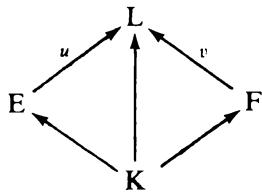
\includegraphics[keepaspectratio]{images/part001_6a404f81.jpg}}\\
图1。

按照一般定义（E，IV，第 6 页），E 和 F 的复合扩张 \((L, u, v)\) 到 E 和 F 的复合扩张 \((L', u', v')\) 上的一个同构是一个 K-同构 \(\varphi\)，它把 L 映到 \(L'\) 上，使得 \(u' = \varphi \circ u\) 且 \(v' = \varphi \circ v\) 。

设 \((\mathbf{L}, u, v)\) 是 \(\mathbf{E}\) 与 \(\mathbf{F}\) 的一个复合扩张。K-线性映射 \(w\)（从 \(\mathbf{E} \otimes_{\mathbf{K}} \mathbf{F}\) 到 \(\mathbf{L}\) 中）把 \(x \otimes y\) 映为 \(u(x)v(y)\)，它是一个 K-代数同态；在本节中，我们把它记作 \(u * v\) 。其像是 \(\mathbf{L}\) 中由 \(u(\mathbf{E}) \cup v(\mathbf{F})\) 生成的子环。

命题 4. --- 设 E、F 是 K 的两个扩张。

\begin{enumerate}
\def\labelenumi{\alph{enumi})}
\item
  设 \((\mathbf{L}, u, v)\) 是 \(\mathbf{E}\) 与 \(\mathbf{F}\) 的一个复合扩张；则 \(\mathfrak{p}\) 是一个素理想，它是同态 \(u * v\)（从 \(\mathbf{E} \otimes_{\mathbf{K}} \mathbf{F}\) 到 \(\mathbf{L}\) 中）的核。
\item
  设 \(\mathfrak{p}\) 是 \(E \otimes_{K} F\) 的一个素理想；则存在一个复合扩张 \((L, u, v)\) （\(E\) 与 \(F\) 的），使得 \(\mathfrak{p}\) 是 \(u * v\) 的核，且任意两个这样的复合扩张都是同构的。
\end{enumerate}

断言 a) 由环到域的同态的核是素理想这一事实得出（I，第 116-117 页）。

设 \(\mathfrak{p}\) 是 \(E \otimes_{K} F\) 的一个素理想，\(A\) 为商环 \((E \otimes_{K} F)/\mathfrak{p}\)，\(L\) 为 \(A\) 的分式域。对 \(x \in E\)（相应地 \(y \in F\)），我们用 \(u(x)\)（相应地 \(v(y)\)）表示在模 \(\mathfrak{p}\) 下 \(x \otimes 1\)（相应地 \(1 \otimes y\)）的剩余类。则 \(u\)（相应地 \(v\)）是 \(E\)（相应地 \(F\)）到 \(L\) 中的 K-同态，且 \(u(E) \cup v(F)\) 生成 \(A\)（作为环），因此生成 \(L\)（作为域）。因此 \((L, u, v)\) 是 \(E\) 与 \(F\) 的一个复合扩张；我们立刻看出 \(u * v\) 是 \(E \otimes_{K} F\) 到 \(L\) 中的典范同态，因此其核等于 \(\mathfrak{p}\) 。

设 \((L', u', v')\) 是 E 和 F 的一个复合扩张，使得 \(u' * v'\) 的核等于 p。由于 \(u * v\) 与 \(u' * v'\) 具有相同的核，存在一个同构 \(\psi\) ，它把 A 映到 \(u' * v'\) 的像 A' 上，由 \(u' * v' = \psi \circ (u * v)\) 刻画。但 A' 是由 \(u'(E) \cup v'(F)\) 生成的 L' 的子环，因此 \(L'\) 是 \(A'\) 的分式域。所以 \(\psi\) 扩张为一个同态 \(\varphi\) （把 L 映到 \(L'\) 上），并且显然 \(\varphi\) 是 \((L, u, v)\) 到 \((L', u', v')\) 上的一个同构。

注记。--- 若 p 和 \(p'\) 是 \(E \otimes_{K} F\) 的两个不同素理想，则对应的 E 与 F 的复合扩张（按上述证明的步骤构造）并不同构。然而，它们作为 K 的扩张仍可能同构（见 V，第 146 页，习题 2）。

推论. --- 存在 E 与 F 的复合扩张。

因为交换环 \(E \otimes_{K} F\) 不化为 0，则它有素理想：克鲁尔定理（I，第 104 页）证明了极大理想的存在性，且每个极大理想都是素理想。

我们可以如下更精确地表述这个推论。设 \((\mathrm{E}, u)\) 与 \((\mathrm{F}, v)\) 是 K 的两个扩张；选取交换环 \(E \otimes_{K} F\) 的一个极大理想 m，并令 \(L = (E \otimes_{K} F)/m\)；则 L 是 K 的一个扩张。对 \(x \in E\)，记 \(u'(x)\) 为 \(x \otimes 1 \mod m\) 的剩余类，并类似地，记 \(v'(y)\) 为 \(1 \otimes y \mod m\) 的剩余类（对所有 \(y \in F\)）。于是我们有以下域同态的交换图

\pandocbounded{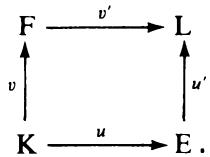
\includegraphics[keepaspectratio]{images/part001_e6455da9.jpg}}

通过把 \((L, u')\) 替换为 E 的一个同构扩张，我们可以假设 L 包含 E 作为子域，并且 \(u'\) 是 E 在 L 中的典范单射。通过更换记号，我们由此得到如下附注：

附注。--- 设 K 与 E 为两个域，且 u 为 K 到 E 的一个同态。若 K' 为包含 K 作为子域的域，则存在一个包含 E 作为子域的域 E'，以及 K' 到 E' 的一个同态 u'，它扩张 u。
% semantic-fragments: legacy-input-seam
\relax{}
